
\documentclass[paper=a4, fontsize=11pt]{scrartcl} % A4 paper and 11pt font size

\usepackage[T1]{fontenc} % Use 8-bit encoding that has 256 glyphs
\usepackage{fourier} % Use the Adobe Utopia font for the document - comment this line to return to the LaTeX default
\usepackage[english]{babel} % English language/hyphenation
\usepackage{amsmath,amsfonts,amsthm} % Math packages
\usepackage{graphicx} % Required for box manipulation
\usepackage{subfigure}
\usepackage{lipsum} % Used for inserting dummy 'Lorem ipsum' text into the template

\usepackage{sectsty} % Allows customizing section commands
\allsectionsfont{\centering \normalfont\scshape} % Make all sections centered, the default font and small caps

\usepackage{fancyhdr} % Custom headers and footers
\pagestyle{fancyplain} % Makes all pages in the document conform to the custom headers and footers
\fancyhead{} % No page header - if you want one, create it in the same way as the footers below
\fancyfoot[L]{} % Empty left footer
\fancyfoot[C]{} % Empty center footer
\fancyfoot[R]{\thepage} % Page numbering for right footer
\renewcommand{\headrulewidth}{0pt} % Remove header underlines
\renewcommand{\footrulewidth}{0pt} % Remove footer underlines
\setlength{\headheight}{13.6pt} % Customize the height of the header

\numberwithin{equation}{section} % Number equations within sections (i.e. 1.1, 1.2, 2.1, 2.2 instead of 1, 2, 3, 4)
\numberwithin{figure}{section} % Number figures within sections (i.e. 1.1, 1.2, 2.1, 2.2 instead of 1, 2, 3, 4)
\numberwithin{table}{section} % Number tables within sections (i.e. 1.1, 1.2, 2.1, 2.2 instead of 1, 2, 3, 4)

\setlength\parindent{0pt} % Removes all indentation from paragraphs - comment this line for an assignment with lots of text

%----------------------------------------------------------------------------------------
%	TITLE SECTION
%----------------------------------------------------------------------------------------

\newcommand{\horrule}[1]{\rule{\linewidth}{#1}} % Create horizontal rule command with 1 argument of height


\title{
\normalfont \normalsize
\textsc{} \\ [25pt] % Your university, school and/or department name(s)
\horrule{0.5pt} \\[0.4cm] % Thin top horizontal rule
\huge Gestionale Aziendale \textit{Union Service} \\ % The assignment title
\horrule{2pt} \\[0.5cm] % Thick bottom horizontal rule
}

\author{Dr. Nicola Pancheri}
\date{\normalsize\today} % Today's date or a custom date

\begin{document}

\maketitle % Print the title
\tableofcontents
\newpage

\section{Requisiti}

%------------------------------------------------

Si vuole realizzare un sistema informativo per gestire le informazioni relative all'attivit\'a svolta
dall'azienda di ristrutturazioni \textit{Union Service};
i dipendenti faranno accesso a tal sistema tramite
un'applicazione appositamente realizzata.\\
L'applicazione sar\'a una web-app (accessibile tramite browser) il cui scopo
principale \'e quello di migliorare la produttivit\'a dei singoli dipendenti,
semplificando le fasi del lavoro che richiedono l'utilizzo del computer,
 e migliorare la comunicabilit\'a e il coordinamento tra uffici;
i dipendenti dovranno essere in grado di accedervi anche da casa.
Il database verr\'a memorizzato su due unit\'a di memoria ( una
delle quali con lo scopo di backup ) e, successivamente,
 su un apposito server online che offre un servizio DBMS cloud
 (database as a service, DBaas).\\

\subsection{I dipendenti}

Nell'azienda distinguiamo quattro classi di dipendenti in
base all'ufficio d'appartenenza o alla mansione svolta:
\begin{itemize}
	\item Commerciale;
	\item Tecnico;
	\item Capo-Cantiere;
	\item Contabile.
\end{itemize}

Un dipendente, a seconda della classe d'appartenenza, pu\'o avere accesso solo ad un gruppo ristretto di informazioni e funzionalit\'a.\\
Ogni dipendete, a prescindere dalla classe d'appartenenza, pu\'o essere un \textit{dipendente autonomo}: la differenza
sta nel fatto che, per i \textit{dipendenti autonomi}, va registrato anche il numero di partita IVA.\\
Oltre a questa classificazione, un dipendente, a prescindere dalla classe d'appartenenza e se \'e autonomo, pu\'o essere anche un
\textit{dirigente}.

\subsubsection{Il dirigente}
Il \textit{dirigente} \'e un dipendente che, oltre ad avere a disposizione le funzionalit\'a e i permessi sui dati
propri della classe a cui appartiene, ha a disposizione funzionalit\'a aggiuntive.\\
In particolare:
\begin{itemize}
    \item \'e l'unico a poter registrare/cancellare un dipendente;
    \item ha il potere di aggiungere note nella sezione \textit{Note dirigente} di un qualsiasi dipendente;
    \item \'e l'unico a poter settare il calendario degli eventi aziendali;
    \item ha il potere di visualizzare le agende di tutti i dipendenti;
    \item deve poter aver accesso a tutte le conversazioni tra utenti;
    \item deve poter ricercare qualunque dipendente registrato e vederne la \textit{Pagina Profilo};
    \item deve poter modificare i dati di registrazione di ogni dipendente in qualunque momento;
    \item per ogni cliente, deve avere accesso ad una pagina che gli mostra il progresso dei lavori (dall'arrivo alla consegna).
\end{itemize}

La ricerca di un dipendente da parte di un \textit{dirigente} verr\'a effettuata in una sezione apposita tramite una
barra di ricerca; il risultato della ricerca ritorner\'a la \textit{Pagina Profilo} del dipendente cercato.
Tale pagina, rispetto alla \textit{Pagina Profilo} personale, da la possibilit\'a di:
\begin{itemize}
 \item modificare i campi inseriti in fase di registrazione;
 \item vedere le \textit{Ferie confermate};
 \item visualizzare le \textit{Note attive} e  lo \textit{Storico delle note}.
 \item visualizzare lo \textit{Storico conversazioni} ovvero tutte le conversazioni degli ultimi 30 giorni
    del dipendente cercato;
\end{itemize}

Nella sezione \textit{Note attive} il \textit{dirigente} potr\'a visualizzare tutte
le note \textit{personali} e \textit{imposte} attualmente disponibili al dipendente; nella sezione
\textit{Storico delle note}, si accede alle note passate (personali e imposte) del dipendente, non pi\'u disponibili
a quest'ultimo ma ancora salvate nel sistema (vedisi sezione "Note").

\subsection{Registrazione e accesso}
I dipendenti, per accedere alle funzionalit\'a dell'applicazione e ai dati contenuti
nel database, dovranno prima essere registrati.\\
Per registrare un nuovo dipendente, un \textit{dirigente}
dovr\'a accedere ad una sezione chiamata \textit{Genera Credenziali} della pagina \textit{Gestione Dipendenti}:
in tale sezione il \textit{dirigente} dovr\'a specificare
la classe del nuovo dipendente e se il nuovo dipendente \'e un dirigente o meno; alla conferma di quanto inserito, il
sistema generer\'a un \textit{Utente Fittizio} e ritorner\'a al \textit{dirigente} un nome utente ed una password
che si incaricher\'a di comunicare al nuovo dipendente.\\\\
Un  \textit{utente fittizio} \'e un particolare tipo di utente dell'applicazione per cui vengono registrati unicamente
username e password e che ha il solo potere di registrare un dipendente.\\
Un \textit{utente fittizio} pu\'o essere creato solo da un \textit{dirigente} attraverso la sezione \textit{Genera Credenziali}
e username e password vengono generati in maniera randomica dal sistema.\\
Ad \textit{utente fittizio} che accede al sistema viene presentata unicamente la \textit{Pagina di Registrazione}.\\
La \textit{Pagina di Registrazione} \'e un form composto da i seguenti campi:
\begin{itemize}
	\item Nome;
	\item Cognome;
	\item Sesso;
	\item Data di nascita;
	\item Codice Fiscale;
    \item Username;
    \item Password;
	\item foto personale;
	\item indirizzo;
	\item telefono;
	\item email;
    \item password email (necessaria per poter inviare email col proprio account);
	\item IBAN;
	\item Disponibilit\'a settimanale (elenco giorni lavorativi della settimana)
	\item numero partita IVA (se dipendente \textit{Autonomo});
\end{itemize}

Alla conferma della registrazione il sistema generer\'a un nuovo \textit{dipendente}, eliminer\'a
l'\textit{utente fittizio} e invier\'a una \textit{nota automatica} al \textit{dirigente}
che ha generato le credenziali per questo specifico \textit{utente fittizio}; tale nota informer\'a il dirigente
dell'avvenuta registrazione del dipendente e gli ricorder\'a di controllare i campi inseriti e di completare i campi
di propria competenza. Infatti, per ogni nuovo \textit{dipendente} registrato, il dirigente deve specificare attraverso
un'apposita sezione, accessibile dalla pagina \textit{Gestione Dipendenti}, le seguenti informazioni:
\begin{itemize}
	\item Tipologia Contratto (determinato o indeterminato);
	\item Scadenza Contratto;
	\item Orario di Lavoro (full-time o part-time);
	\item Costo Orario;
\end{itemize}


Ogni \textit{dipendente} pu\'o riaccedere in qualunque momento alla \textit{Pagina Profilo}
per visualizzare/modificare le informazioni inserite in fase di registrazione come \textit{utente fittizio}.

\subsection{Funzionalit\'a comuni}

Confermata la correttezza delle credenziali inserite
nella \textit{Pagina d'accesso}, il sistema presenta al dipendente la sua \textit{Homepage};
come specificato in precedenza, l'\textit{Homepage} \'e personalizzata in base alla classe d'appartenenza del dipendente.\\
Tramite l'applicazione, a prescindere dall'ufficio d'appartenenza, i dipendenti devono:
\begin{itemize}
\item avere a disposizione una \textit{pagina profilo};
\item essere in grado di comunicare tra loro tramite una chat;
\item avere a disposizione un'agenda personale;
\item avere a disposizione un calendario per viusalizzare gli eventi aziendali ( ferie, chiusure particolari, etc. );
\item avere a disposizione una sezione per poter impostare le proprie ferie;
\item avere un modo rapido di settare/visualizzare note;
\item poter cercare velocemente un cliente tramite un'apposita barra di ricerca.
\end{itemize}

Le conversazioni delle chat devono rimanere registrate nel sistema 30 giorni prima di essere rimosse.

\subsubsection{La pagina profilo}
Attraverso la propria \textit{Pagina profilo} un dipendente pu\'o visualizzare i propri dati personali
registrati nel sistema e modificare i dati inseriti al primo accesso;
un dipendente non pu\'o modificare i dati inseriti in fase di registrazione dal \textit{dirigente}.\\
Dalla pagina profilo devono essere anche impostabili le proprie ferie annuali.

\subsubsection{Il calendario aziendale}

Tramite un apposito link in \textit{Homepage}, ogni dipendente deve avere accesso al \textit{calendario aziendale}.
Il \textit{calendario aziendale} \'e un calendario suddiviso per mesi in cui \'e possibile visualizzare gli \textit{eventi aziendali};
tali eventi possono essere impostati solamente da un \textit{dirigente} che avr\'a a disposizione tale funzionali\'a attraverso
la propria sezione \textit{calendario aziendale}.\\
Un \textit{evento aziendale}  ha un titolo ed \'e associato ad un particolare mese e giorno.\\

Un \textit{dipendente} vedr\'a, nel proprio \textit{calendario aziendale}, una tabella, dove, ad ogni cella
corrisponde un mese; gli eventi associati ad un determinato mese appariranno elencati nella cella associata al mese
e ordinati in base al giorno con cui son stati registrati.



\subsubsection{Le ferie}
Le ferie sono impostabili dalla \textit{Pagina profilo}; per ogni periodo di vacanze che si vuole impostare,
il \textit{dipendente} deve inserire la durata, il primo giorno di vacanza (inteso come giorno e mese) e un titolo (opzionale).\\
Al termine della compilazione, si generer\'a un'apposita nota ai \textit{dirigenti}: le ferie impostate da un dipendente
\textit{non-dirigente} saranno effettivamente registrate solo dopo che un qualsiasi \textit{dirigente} le avr\'a confermate.
Le ferie confermate, saranno visualizzabili solo dal dipendente che le ha richieste nel proprio \textit{calendario aziendale}
 assieme agli eventi aziendali( ma appositamente differenziate ).

Nella propria sezione \textit{Note}, i \textit{dirigenti} avranno un apposita sottosezione \textit{ferie da confermare}
in cui vengono elencate tutte le \textit{richieste di ferie}; selezionando una di queste \textit{richieste di ferie}
il \textit{dirigente} potr\'a o confermarla o negarla: in caso di negazione, sar\'a data la possibilit\'a di aggiungere
una nota.

Alla conferma o negazione di una \textit{richiesta di ferie}, al dipendente che ha fatto richiesta, comparir\'a una
nota specifica.


\subsubsection{Le note}

Le \textit{note} che verranno visualizzate da un \textit{dipendente} in \textit{Homepage} sono di tre tipi:
\textit{personali}, \textit{imposte} e \textit{automatiche}; le \textit{note imposte} a loro volta possono
essere \textit{confermate} o \textit{non-confermate}.\\
Le note \textit{personali} sono quelle settate dal dipendente stesso,
le note \textit{imposte} sono settate da un \textit{dirigente} per quel dipendente,
le note \textit{automatiche} sono generate dal sistema;\\
un esempio di note automatiche sono quelle generate alla conferma/negazione di una \textit{richiesta di ferie}.\\
Per ogni \textit{Nota}, viene memorizzato un titolo e un contenuto (opzionale).
A fianco di ogni nota, deve essere possibile fare un segno di spunta; a termine giornata tutte le \textit{note spuntate}
verranno rimosse dall'elenco delle note da visualizzare.\\\\
Le \textit{note imposte} hanno un meccanismo proprio diverso:
un \textit{dirigente} invia una \textit{nota imposta} ad un \textit{dipendente}; a seguito di ci\'o, la \textit{nota imposta}
comparir\'a nell'apposita sezione del \textit{dipendente} e nella sezione \textit{Note non-confermate} del dirigente.
Alla conferma di una \textit{nota imposta}, il \textit{dipendente} sar\'a obbligato ad aggiungere un commento.
La conferma di una \textit{nota imposta} avr\'a come effetto l'eliminazione della nota tra l'elenco delle \textit{note non-confermate}
del \textit{dirigente} che l'aveva generata e l'invio, allo stesso \textit{dirigente}, di una \textit{nota automatica}
avente come contenuto il commento lasciato dal \textit{dipendente}.\\\\
Le note \textit{personali} e \textit{imposte} seppur spuntate o confermate dovranno rimanere memorizzate nel sistema per un periodo
di tempo di 6 mesi.

\newpage
\subsection{Il cliente}
Nel applicazione distinguiamo cinque tipologie di clienti: \textit{accolto},
\textit{preventivato}, \textit{in lavorazione}, \textit{perso}, \textit{vecchio}.\\
All'arrivo in azienda, un cliente si interfaccia in primoluogo con l'\textit{ufficio commerciale}:
in questa fase, il commerciale che lo accoglie registra nel sistema il cliente come \textit{cliente accolto}.
Nello stesso momento o in uno successivo, il cliente e il commerciale potrebbero decidere di stilare un preventivo:
al termine della compilazione del preventivo il cliente diventa di tipo \textit{preventivato}.\\
Un \textit{cliente preventivato} potrebbe ancora rifiutare il lavoro: solo topo la stesura del contratto il cliente diventa
\textit{in lavorazione} altrimenti il cliente diventa \textit{perso}.\\
Un cliente per cui \'e stata completato un \textit{lavoro} diventa \textit{vecchio}; ad un \textit{cliente vecchio}
deve essere possibile associare pi\'u \textit{lavori}.\\
Ogni cliente dal momento in cui viene registrato possiede una \textit{Pagina Cliente} da cui
ogni dipendente potr\'a accedere a funzioni dell'applicazione specifiche per lavorare con quel cliente, ad esempio: la
\textit{Pagina preventivo}, la \textit{Pagina contratto}, la \textit{Pagina avanzamento lavori}, ecc.

Per ogni cliente va registrato: nome, cognome, indirizzo, telefono, email, dati sopralluogo,
rilievo sopralluogo, archivio foto ( suddiviso in: prima dei lavori, avanzamento lavori,
completamento lavori), planimetrie catastali, preventivo commerciale, preventivo
finiture, contratto, cronoprogramma, ordini, identificativi dei dipendenti che lavorano
col cliente.
Gran parte delle informazioni vengono inserite a mano a mano che i lavori procedono.


\subsection{Funzionalit\'a accessibili dall'\textit{ufficio commerciale}}

Tramite l'applicazione, i dipendenti che lavorano nell'ufficio commerciale
devono poter:
\begin{itemize}
    \item aggiungere un nuovo cliente;
    \item togliere un vecchio cliente;
    \item compilare in maniera semplice il preventivo del cliente;
    \item compilare il contratto per il cliente;
    \item aggiungere/togliere/modificare le voci del database riguardanti il preventivo;
    \item compilare il \textit{modulo gradimento lavori}.
\end{itemize}

\subsubsection{Registrazione cliente}
Ogni commerciale pu\'o registrare nel sistema un cliente come \textit{accolto}
tramite la pagina \textit{Registrazione Cliente}.\\
In tale pagina viene presentato un form con i seguenti campi da compilare:
\begin{itemize}
    \item nome e cognome del cliente;
    \item indirizzo del cliente;
    \item un campo di testo "libero" in cui il commerciale si annota il tipo di lavoro richiesto;
    \item un grado di difficolt\'a del cliente da 1 a 3;
    \item una tipologia di cliente tra: immobiliare, privato, azienda;
    \item referenza: passaparola, fiera, ufficio, internet o altro.
\end{itemize}

Oltre a ci\'o, il sistema richieder\'a se per il lavoro richiesto \'e necessario fare un sopraluogo:
in caso di risposta affermativa, si dovr\'a impostare l'appuntamento per il sopraluogo attraverso la \textit{Pagina sopraluogo},
accessibile dalla pagina \textit{Registrazione Cliente}.\\
Per vari motivi, i dati per l'appuntamento potrebbero non essere subito noti: al commerciale deve essere data
la possibilit\'a di impostarli in un secondo momento; se il commerciale decide impostarli in un secondo momento,
il sistema generer\'a una \textit{nota automatica} che gli ricorder\'a, i giorni successivi, di dover impostare
l'appuntamento con quel cliente.
Attraverso questa nota dev'essere possibile riaprire la \textit{Pagina sopraluogo} per quel cliente.\\
\'E possibile che il commerciale subito dopo la registrazione del cliente voglia preventivarlo subito:
dalla pagina \textit{Registrazione} deve essere possibile accedere alla pagina \textit{Preventivo}.
Se non \'e necessario alcun sopraluogo e il preventivo viene rimandato, il sistema obbligher\'a il
commerciale a inserire una data indicante entro quando fare il preventivo: dal giorno indicato in poi, apparir\'a
una \textit{nota automatica} che ricorda al commerciale di fare il preventivo per quel cliente.

\subsubsection{Pagina sopraluogo}
Nella \textit{Pagina sopraluogo} il commerciale fissa l'appuntamento per il sopraluogo per un dato cliente;
in particolare dovr\'a inserire le seguenti informazioni:
\begin{itemize}
    \item data e ora;
    \item tecnico che accompagna (opzionale);
\end{itemize}

Al termine della compilazione di questa pagina , al commerciale e all'eventuale tecnico comparir\'a in \textit{agenda}
l'appuntamento.
Deve essere possibile modificare in un secondo momento l'appuntamento:
dall'agenda, cliccando sul \textit{evento sopraluogo}, si portanno modificare i dati dell'appuntamento.
Dopo sette giorno dalla data del sopraluogo, al commerciale deve apparire una \textit{nota automatica} che gli
ricorda di dover chiamare il cliente per fare il \textit{preventivo}.

\subsubsection{Il preventivo}
Un preventivo \'e un insieme di \textit{lavorazioni} da compiere per un determinato \textit{lavoro}
e pu\'o venir compilato da un \textit{commerciale} o da un \textit{tecnico} attraverso la \textit{Pagina Preventivo}
accessibile dalla \textit{Pagina Cliente};
ogni \textit{lavorazione} \'e raggruppata in \textit{settori di lavorazione}.\\
 Per ogni \textit{settore di lavorazione} va registrato il nome e una priorit\'a
 ( da cui dipender\'a l'ordine di visualizzazione delle \textit{lavorazioni} nel \textit{preventivo}).\\
Per ogni \textit{lavorazione}  va registrato il nome, un prezzo unitario, il \textit{settore di lavorazione}.\\
Ogni dipendente di tipo \textit{commerciale} o \textit{tecnico} ha il potere di aggiungere/rimuovere \textit{settori di lavorazione},
aggiungere nuove \textit{lavorazioni} ad un settore, spostare una \textit{lavorazione} da un settore ad un altro,
cambiare temporaneamente il settore di default di una lavorazione per un dato preventivo.



Il preventivo ha due modalit\'a di visualizzazione: \textit{cliente} e \textit{dipendente}; la \textit{visualizzazione cliente}
\'e una versione ridotta della \textit{visualizzazione dipendente}.\\

Terminata la compilazione di un preventivo, si procede alla \textit{stampa del preventivo}:
questa fase implica la chiusura del preventivo;
Entro sette giorni dalla chiusura del preventivo, al dipendente responsabile della sua stesura
 deve apparire una \textit{nota automatica} che gli ricorda di chiamare il cliente per la
 compilazione del \textit{contratto}.

Terminata la compilazione del preventivo il sistema calcola il budget
dei lavori; questo budget \'e un'approssimazione: il budget effettivo
vien ricalcolato alla fine del \textit{preventivo finiture}.\\

Entro sette giorni da quando \'e stato effettuato il preventivo per un cliente,
al commerciale che si \'e occupato del cliente deve comparire una nota ben
visibile che ricorda di richiamare il cliente.



\subsection{Funzionalit\'a accessibili dall'\textit{ufficio tecnico}}

Tramite l'applicazione, i dipendenti che lavorano nell'ufficio tecnico
devono poter:
\begin{itemize}
\item compilare in maniera semplice il \textit{preventivo finiture} del cliente;
\item aggiungere/togliere/modificare le voci del database riguardanti il \textit{preventivo finiture};
\end{itemize}

Al termine della compilazione del preventivo, viene generata una lista di oggetti da
ordinare, ricalcolato il budget dei lavori e, infine, vengono inviati all'ufficio capi-cantiere:
\begin{itemize}
\item la lista finiture con le differenze capitolato;
\item le conferme d'ordine con le date di consegna;
\item le schede tecniche dei prodotti ordinati.
\end{itemize}

\subsection{Funzionalit\'a accessibili dall'\textit{ufficio capi-cantiere}}

I dipendenti di tal ufficio usano l'applicazione per:
\begin{itemize}
\item compilare il cronoprogramma;
\item visualizzare il budget di lavoro e la lista degli ordini;
\item caricare foto, rilievi, planimetrie nella pagina di un dato cliente;
\item compilare il modulo varianti.
\end{itemize}

Il cronoprogramma deve essere sempre modificabile e specifica come vengono
gestiti i lavori in cantiere.
In base alla definizione del cronoprogramma vien determinato anche quando effettivamente
effettuare gli ordini specificati dall'ufficio tecnico: un mese prima (tale periodo
deve essere impostabile) che un oggetto serva effettivamente, deve essere inviata
un'email verso l'azienda che lo vende.


\subsection{Schermata \textit{avanzamento lavori}}

Tramite questa funzionalit\'a dell'applicazione, il \textit{responsabile}
deve essere in grado di monitorare il completamento di tutte le attivit\'a
dei vari uffici, dall'arrivo del cliente al completamento dei lavori.

\newpage
\section{Lavori, tempi e costi}

La realizzazione complessiva del sistema si sviluppa nelle seguenti fasi:
\begin{itemize}
\item Progettazione e analisi del database;
\item Implementazione del database;
\item Progettazione dell'applicazione;
\item Implementazione dell'applicazione;
\item Verifica del sistema;
\item Configurazione del server per l'installazione del sistema;
\item Installazione del sistema;
\item Periodo rodaggio.
\end{itemize}

L'intero sistema ha come requisiti da parte dell'azienda:
\begin{itemize}
\item l'avere i computer connessi nella rete aziendale interna;
\item l'avere la rete interna connessa ad Internet (solo per poter avere accesso dall'esterno);
\item l'avere un server connesso alla rete
( preferibile, ma non necessario, con installata una qualsiasi distribuzione server di Linux ).
\end{itemize}

Il completamento del sistema richieder\'a approssimativamente 60 giorni;\\
Il costo preventivato per lo svolgimento complessivo del lavoro (manutenzione nel periodo di rodaggio inclusa)
\'e di 1200 euro, considerando una media lavorativa di 4 ore giornaliere al costo di 5 euro/h.

\newpage

\section{Tecnologie usate}

\section{Documentazione progettazione database}
\subsection*{Modello Concettuale}



    \begin{figure}[htbp]
        \centering
        \subfigure{
          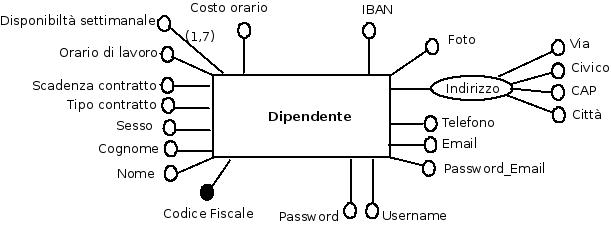
\includegraphics[scale=0.4]{Immagini/ER-dip.jpg}
        }

        \qquad\qquad\qquad\qquad\qquad\qquad\qquad\qquad
        \subfigure{
          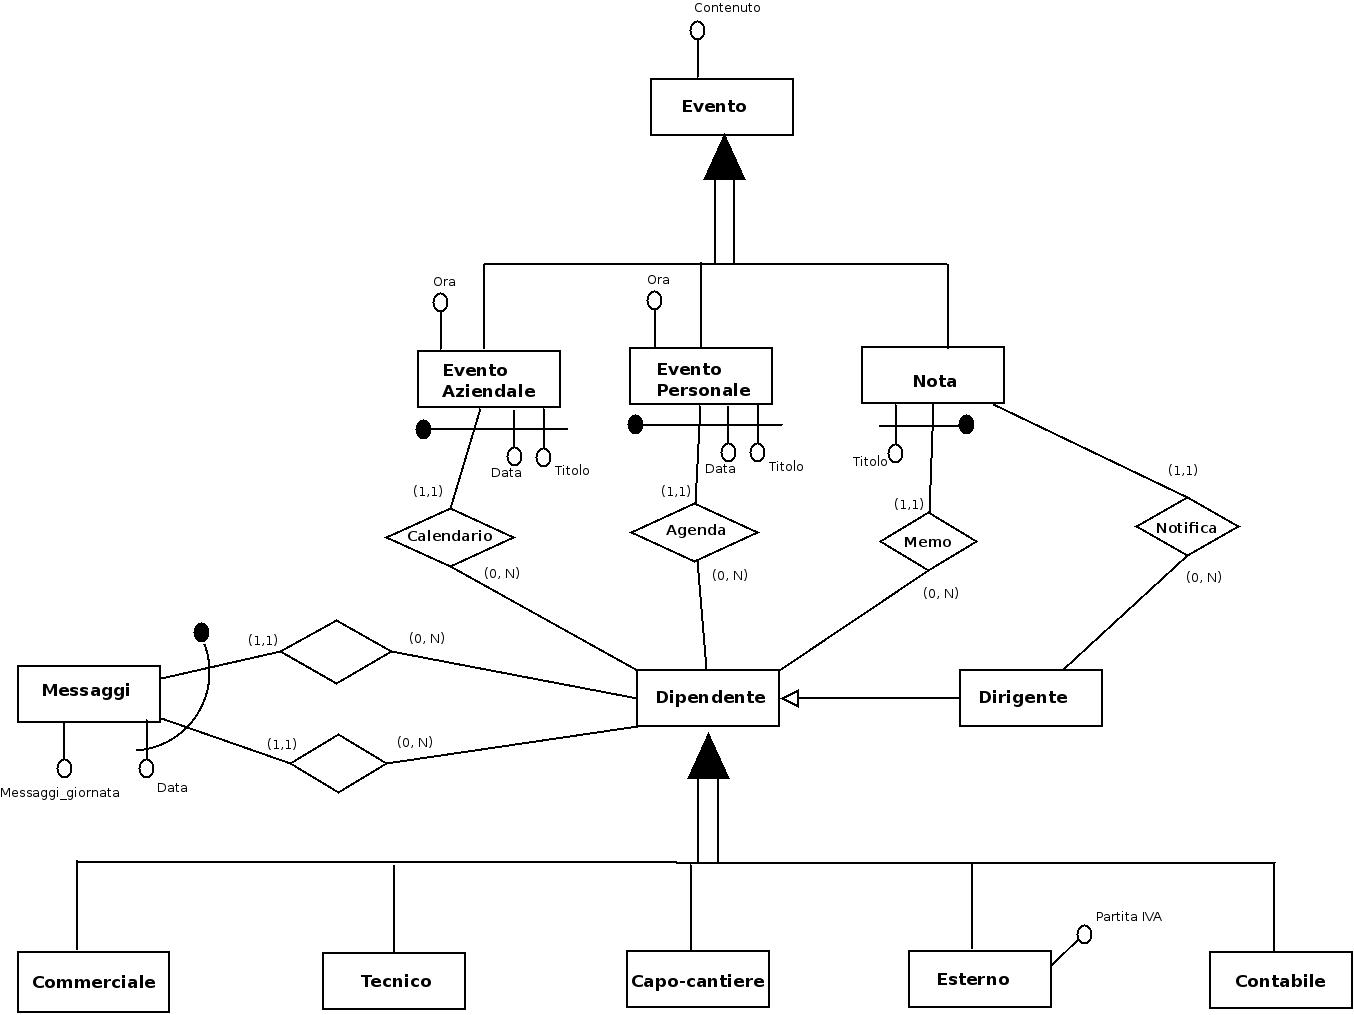
\includegraphics[scale=0.3]{Immagini/ER-completo.jpg}
        }

        \qquad\qquad
      \end{figure}

\newpage
\subsection*{Ristrutturazione del modello concettuale}


    \begin{figure}[htbp]
        \centering
        \subfigure{
          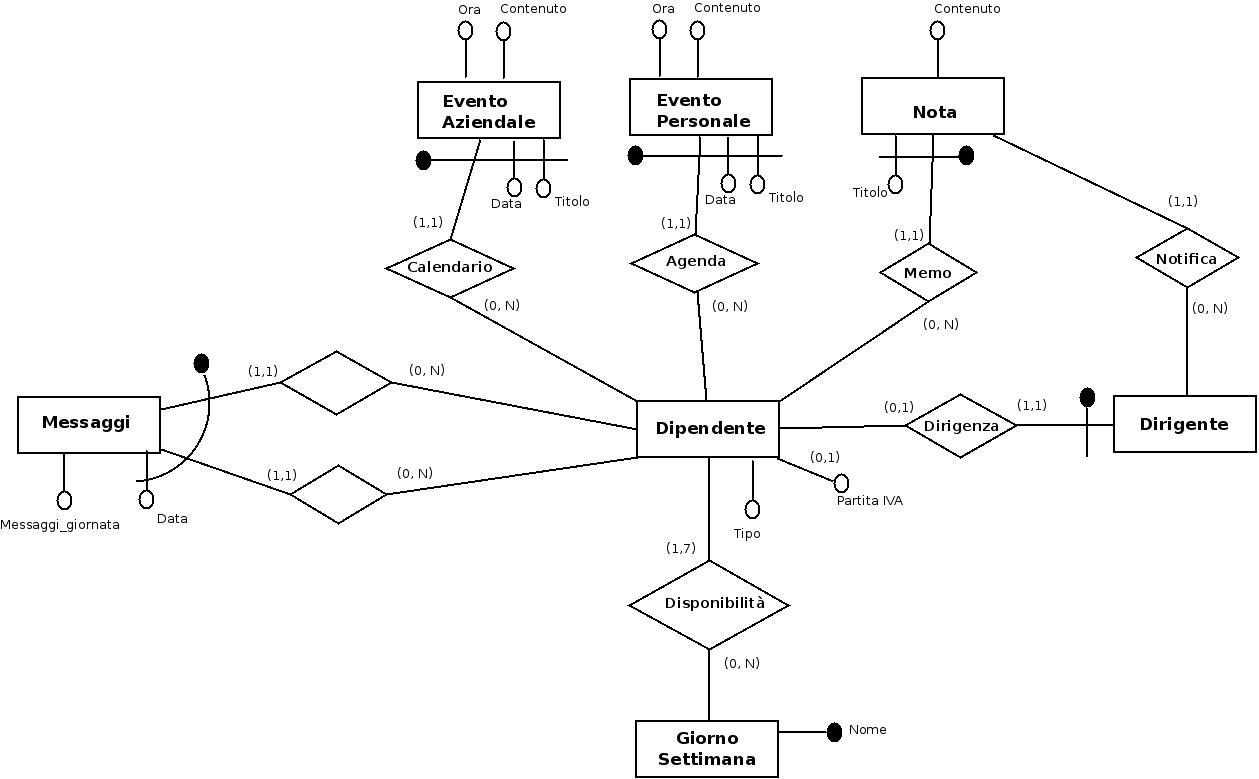
\includegraphics[scale=0.3]{Immagini/ER-ristrutturato.jpg}
        }
        \qquad\qquad
      \end{figure}

\subsection*{Modello Logico}
\begin{itemize}
  \item dipendente(\underline{cf}, username, password, nome, cognome, sesso, via, civico, cap, citta, foto, telefono,
      email, password\_email, tipo\_dipendente, tipo\_contratto, scadenza\_contratto, orario\_lavoro, costo, iban, partita\_iva);
  \item dirigente(\underline{cf});
  \item evento\_aziendale(\underline{data},\underline{titolo}, \underline{dipendente}, ora, contenuto);
  \item evento\_personale(\underline{data},\underline{titolo}, \underline{dipendente}, ora, contenuto);
  \item nota(\underline{titolo}, \underline{dipendente}, dirigente, contenuto);
  \item giorno\_settimana(\underline{nome});
  \item disponibilita(\underline{dipendente}, \underline{giorno});
  \item messaggi( \underline{data}, \underline{dip1}, \underline{dip2}, messaggi\_giornata)

\end{itemize}

\subsubsection*{Superchiavi}

\begin{itemize}
  \item dipendente(username, password);

\end{itemize}



\subsubsection*{Vincoli d'integrit\'a referenziale}

\begin{itemize}

  \item dirigente.cf -> dipendente.cf;
  \item evento\_aziendale.dipendente -> dipendente.cf;
  \item evento\_personale.dipendente -> dipendente.cf;
  \item nota.dipendente -> dipendente.cf;
  \item nota.dirigente -> dirigente.cf;
  \item disponibilita.dipendente -> dipendente.cf;
  \item disponibilita.giorno -> giorno\_settimana.nome;
  \item messaggi.dip1 -> dipendente.cf;
  \item messaggi.dip2 -> dipendente.cf;


\end{itemize}

\newpage
\section{Documentazione progettazione applicazione}


\end{document}
